The containment of the energy in the supercluster was verified
with simulations  performed with
\SRIM~\cite{bib:srim} of nuclear and electron recoils  within the gas mixture of the \lemon detector.
For both types of recoils, for the energy range of interest for DM
 search, \eg $E<10\keV$, when considering deposits without electronics
 noise and no diffusion in the gas, the peak of the
 $\abs{E-E_{true}}/E_{true}$ is within 5\%. Adding a Gaussian noise
 distribution with a mean equal to the one observed in the pedestal
 runs, and a diffusion following the parameterization in
 Eq.~\ref{eq:diff}, the fraction of the true energy contained in the
 supercluster decreases to about 80\%, as shown in
 Fig.~\ref{fig:eoveretrue}. The distributions were obtained for
 nuclear recoils with $E=6\keV$ generated at the exact center of
 the \lemon detector. The mean and the Gaussian width of the peak are
 estimated by fitting the distributions with a Crystal Ball
 shape~\cite{Oreglia:1980cs,Gaiser:1982yw}, which includes a tail to
 consider a non-Gaussian asymmetric tail due to partial containment in
 the supercluster.

The decrease in the energy containment in the supercluster is due to
the smearing of the 2D track pattern around the periphery of the
cluster.  This decreases the gradients in Eq.~\ref{eq:gradient} around
the edges, and so the supercluster can shrink more around the crest,
loosing part of the tails that can be confused more easily with the
noise.  A more realistic noise description, and an improved diffusion
model, based on the one measured in data is necessary to tune the
supercluster parameters in simulation to recover part of the
containment. Despite this, the resolution in presence of noise and
diffusion is estimated in this simulated nuclear recoils with
$E=6\keV$ to be around 4\%. This energy resolution is expected to be
very optimistic because the absence, in the simulation, of the
dominant fluctuations of the GEM gain.
%
\begin{figure}[ht]
  \begin{center} 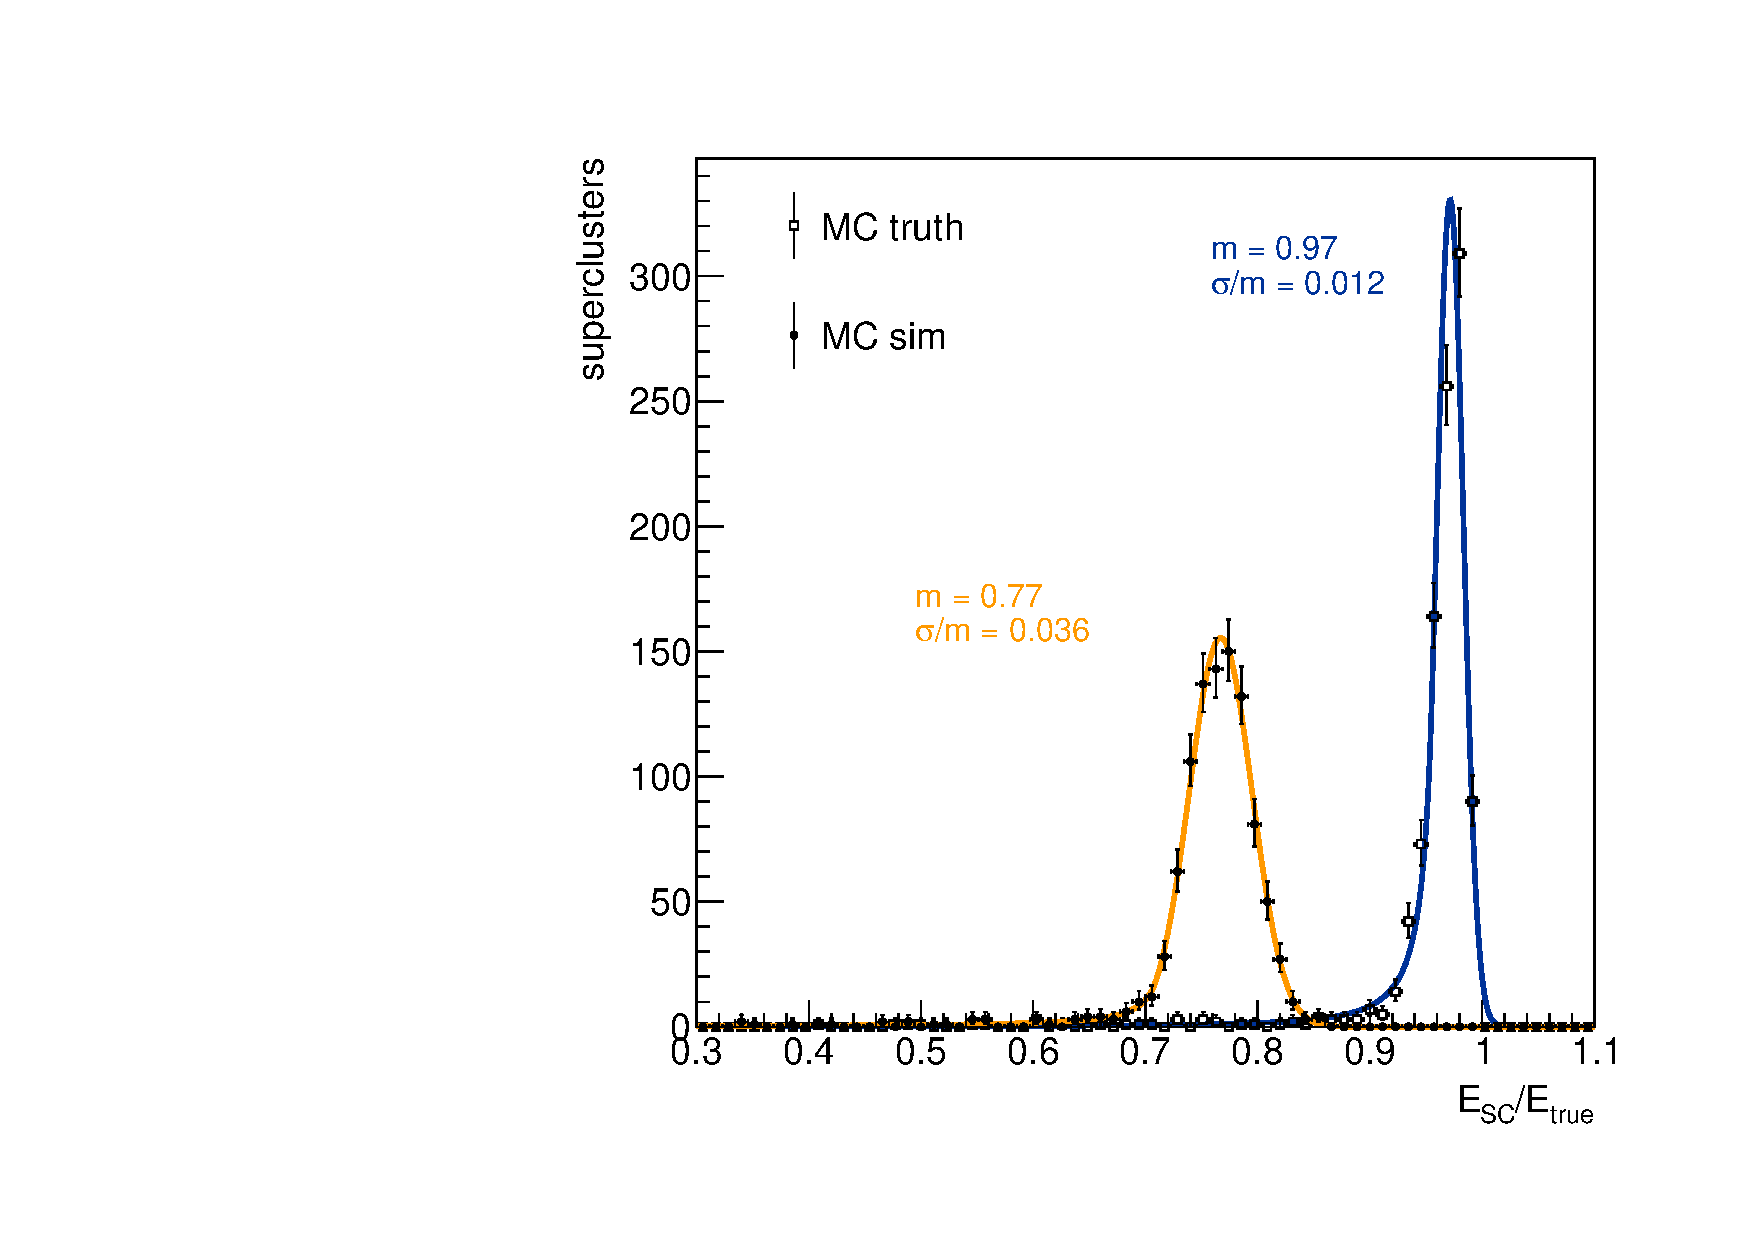
\includegraphics[width=0.49\linewidth]{figures/eoveretrue}
   \caption{Distribution of the ratio of reconstructed supercluster
    energy, $E$, and the true energy of nuclear recoils
    $E_{true}=6\keV$, generated in the center of \lemon and simulated
    with \GEANTfour Monte Carlo (MC). The hollow points show the MC
    events generated without electronics noise and diffusion in the
    gas, while the filled circles represent MC events with both
    effects included. The curves represent parametric fits with a
    Crystal Ball function.\label{fig:eoveretrue}}
  \end{center}
\end{figure}
%

The absolute energy scale was then calibrated with the energy distribution
measured in data with the \fe source, which provides monochromatic
photons of 5.9\keV, with the procedure described in
Ref.~\cite{bib:fe55}. The supercluster integral is defined as:
\begin{equation}
\label{eq:integral}
I_{SC} = \sum_i^{cluster} N_i,
\end{equation}
where $N_i$ is the number of counts (photons) in the $i^{th}$ pixel,
and the sum runs over all the pixels of the supercluster.  While to
perform the basic- and super-clustering only pixels passing the zero
suppression are considered, for the energy estimate in
Eq.~\ref{eq:integral} all the pixels within the cluster contours are
counted, eventually having negative $N_i$, after the pedestal
subtraction. This is done to avoid a bias on the energy estimate.
The distribution of \isclu, for a run taken in presence of \fe source,
is shown in Fig.~\ref{fig:feuncalibpeak}.
%
\begin{figure}[ht]
  \begin{center}
    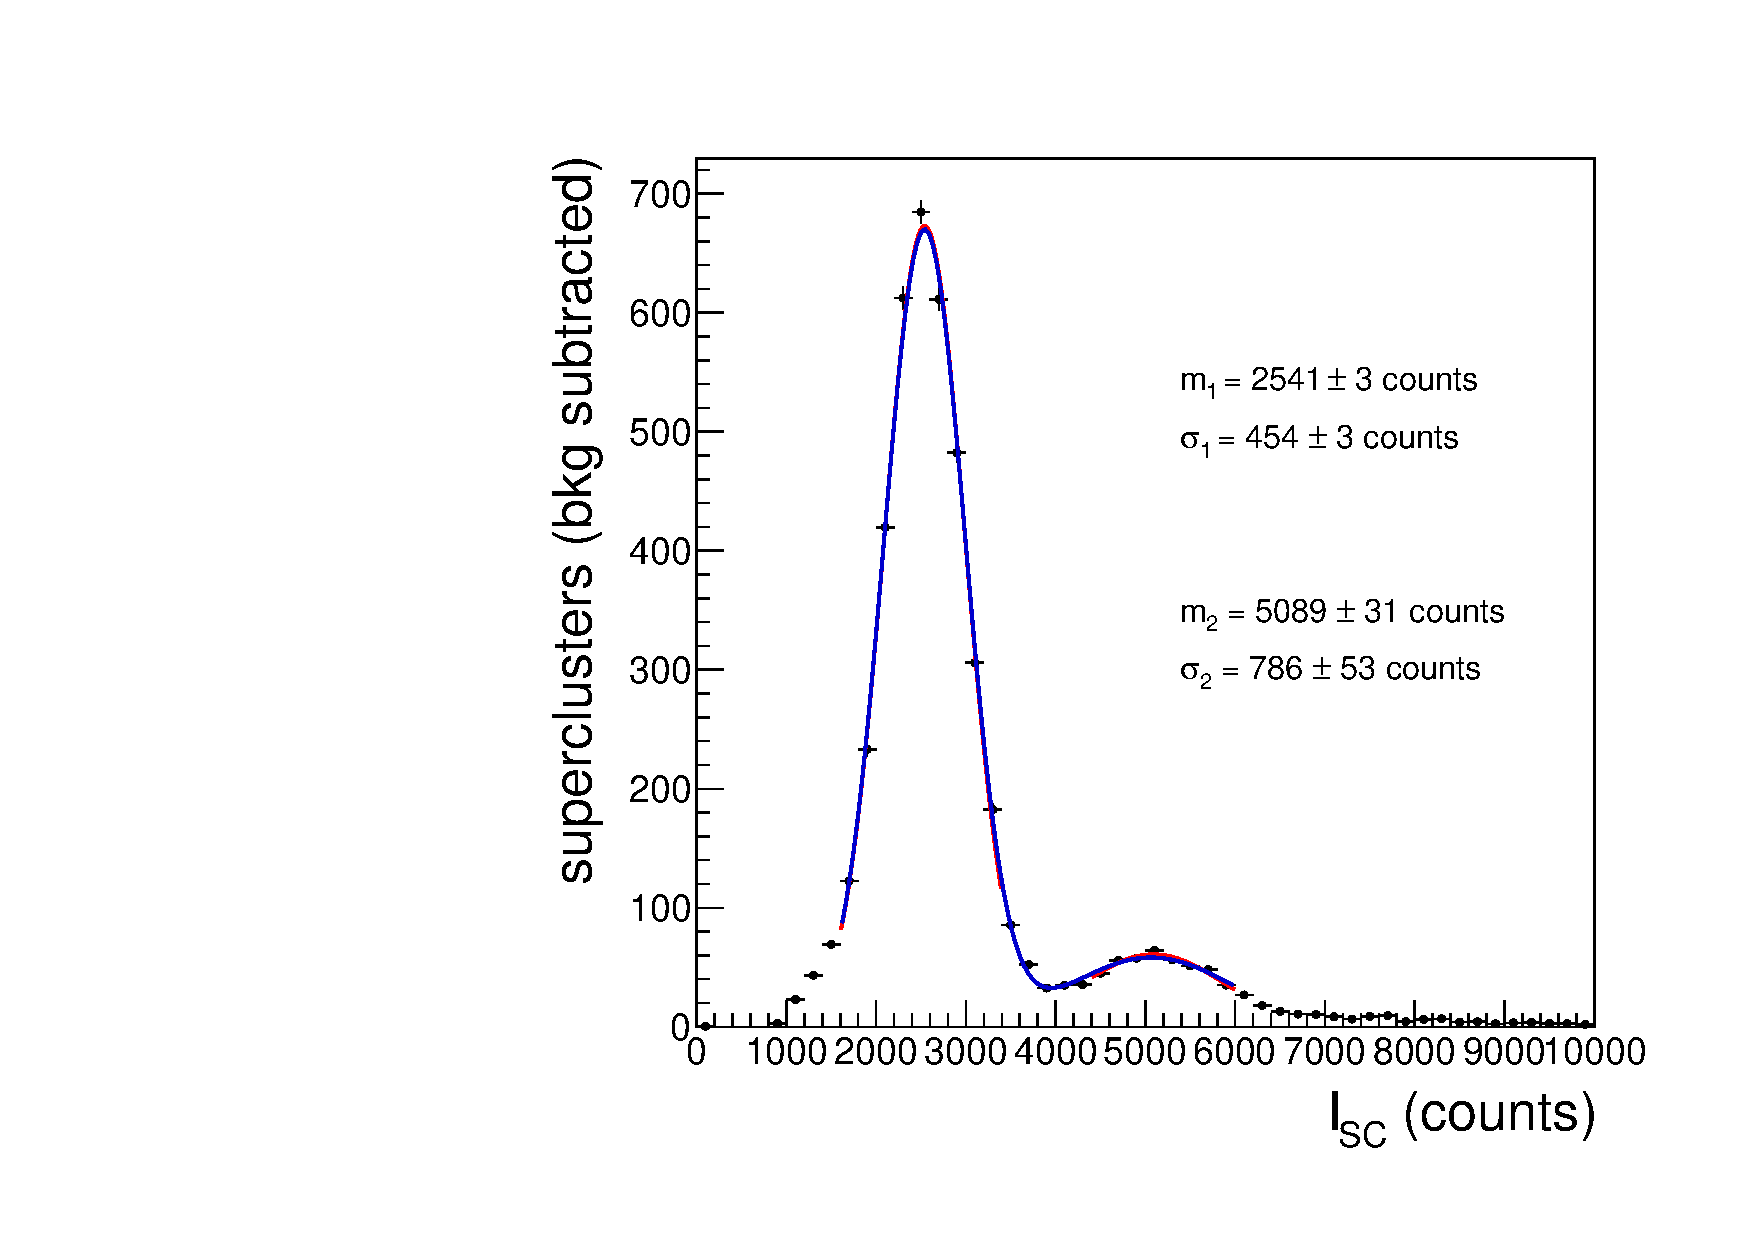
\includegraphics[width=0.49\linewidth]{figures/fe_ucalibintegral_fit}
    \caption{Distribution of the supercluster integral, before the
      absolute energy scale calibration is applied, in events with the
      \fe source. Clearly visible is the large peak of a single spot,
      and, at around twice the energy, a broader peak for the case of
      two neighboring spots merged in a single supercluster.
      \label{fig:feuncalibpeak}}
  \end{center}
\end{figure}
%
 The position of the maximum in the single-spot distribution in runs
with \fe source allowed to calibrate the absolute energy scale of
the \lemon detector.  The energy resolution for the reconstructed \gac
superclusters is about 18\%, similar to the one that can be obtained
with only the basic clustering step with \idbscan~\cite{iDBSCAN}, and
improving the one with the simple \nnc algorithm previously
used~\cite{bib:fe55}. This value is still much larger than the one
obtained with the simulation of nuclear recoils at the same energy,
but an improved noise and gas diffusion model, and a simulation of the
gas gain fluctuations are needed to improve the data-MC agreement.


Using runs with this monochromatic, high rate source, positioned at
different distances from the GEM planes, a decrease of the light
response for lower distances from the GEM was observed. This effect is
opposite to the expected behavior of a decreasing light yield at
larger distances. Indeed, it is expected that during the drift along
the $z$-direction the ionization charge undergoes a diffusion in the
TPC gas and some electrons are removed by attachment to the gas
molecule.  Consequently some loss in the light collection may be
expected. The opposite behavior, instead, is clearly observed. While
this effect is currently under study in more detail, it was attributed
to a possible saturation effect of the GEMs, especially in the third
stage of multiplication, for which the charge density in one GEM hole
is maximal.  Under this hypothesis, an effective, empirical correction
was developed, which relies on the charge density of a cluster from
a \fe deposit. The light density, $\delta$, is defined as:
\begin{equation}
  \label{eq:density}
  \delta = \isclu / n_p,
\end{equation}
where $n_p$ is the number of pixels passing the zero-suppression
threshold (differently from the numerator, where all the pixels in the
supercluster are considered). This effective calibration provides the
absolute energy of a spot-like region similar to the \fe ones, as a
function of the supercluster density, $\delta$: $E=c(\delta)\cdot
I_{SC}$. In the hypothesis of saturation, the
\textit{local} density along the track is the parameter which
regulates the magnitude of the effect, thus the correction has to be
applied dynamically for slices of the supercluster having a size
similar to the \fe spots.  This is achieved with the procedure
described in the following.

First, the supercluster \textit{skeleton}, \ie, the 1 pixel wide
representation along the energy deposition path, is reconstructed.
This is performed with a morphological thinning of the superclusters
with the iterative algorithm from Ref.~\cite{thin1,thin2}.  Second, a
pruning of the obtained skeleton is done, to remove residual branches
along the main pattern, using a hit-or-miss transform.  The output of
the \textit{skeletonization} for the track of
Fig.~\ref{fig:super_clusters1} is shown in Fig.~\ref{fig:skeleton}.
%
\begin{figure}[ht]
  \begin{center}
     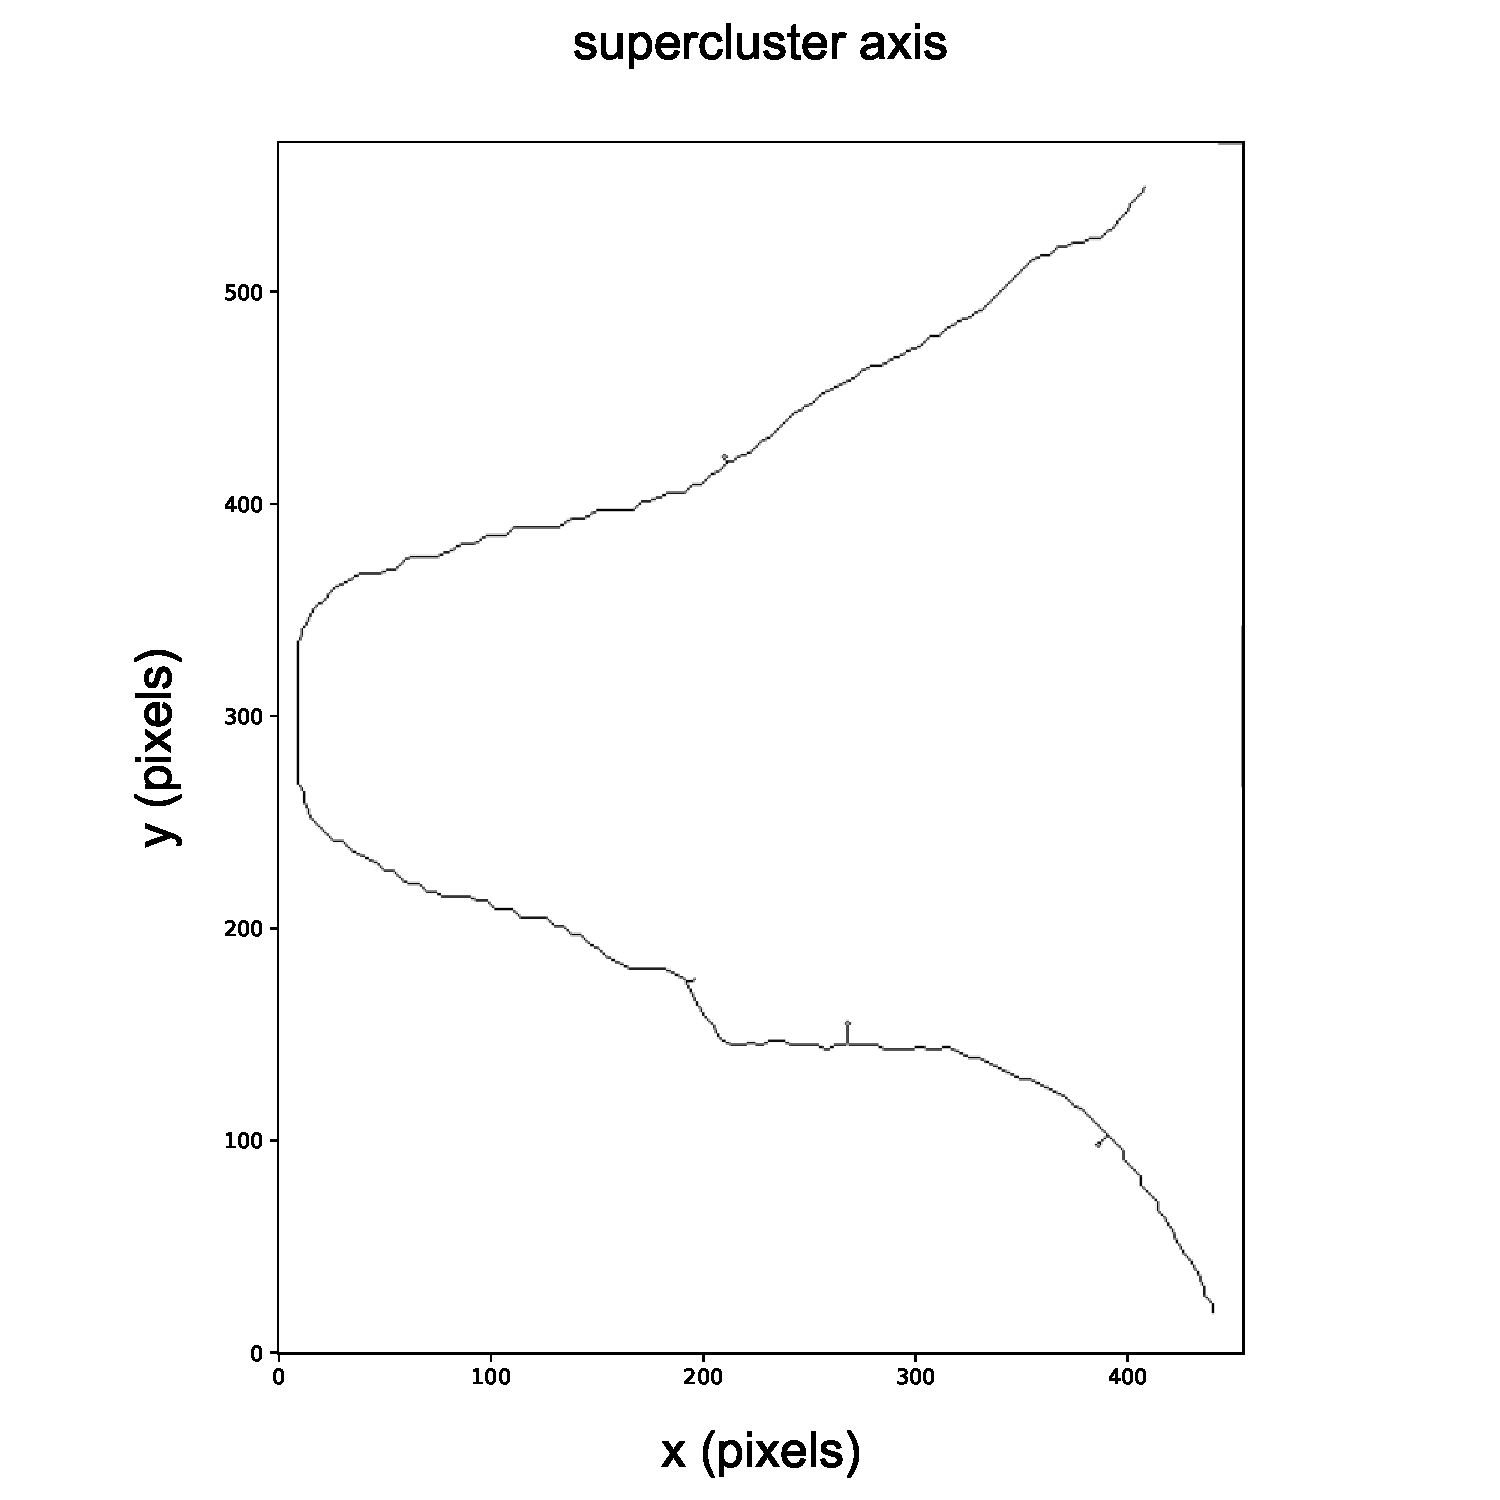
\includegraphics[width=0.49\linewidth]{figures/skeleton_paper}
     \caption{Output of the skeletonization and pruning of the
       branches for one example supercluster extended in
       space.  \label{fig:skeleton}}
  \end{center}
\end{figure}
%
For the calibration procedure, the skeleton was followed, starting
from one of the two end points, and circles having their center on a
pixel of the skeleton and their radius equal to the average spot size
of the \fe clusters were defined. The local density $\delta_s$ of the
slice $s$ is computed, and its integral $I_s$ is calibrated to an
absolute energy through the effective correction $E_s=c(\delta_s)\cdot
I_s$. The pixels of the supercluster used for the slice calibration
are removed (including the skeleton ones), and the procedure is
iterated, until having included all the pixels. The sum of the
energies of all the slices is the estimate of the calibrated energy of
the supercluster:
%
\begin{equation}
  \label{eq:ecal}
  E_{SC} = \sum_s^{slices} E_s
\end{equation}
%
As a closure test of this procedure, the calibrated energy of the
superclusters reconstructed in the runs with the \fe source is
obtained.  The value of the energy peak was obtained by fitting the
distribution with the same function used in
Fig.~\ref{fig:feuncalibpeak}, and equals to  $m_1 = 5.93 \pm 0.01$\keV,
compatible with the expected value. The calibration procedure is an
overkill for the case of the small \fe spots, but it is necessary for
very long cosmic ray tracks or even for medium-length superclusters
from nuclear and electron recoils.  The energy resolution worsen after
the calibration ($\sigma_1 = 1.48 \pm 0.01$, \ie, 25\% energy
resolution), as a sign that the empiric correction is still
suboptimal.
%
%% \begin{figure}[ht]
%%   \begin{center}
%%     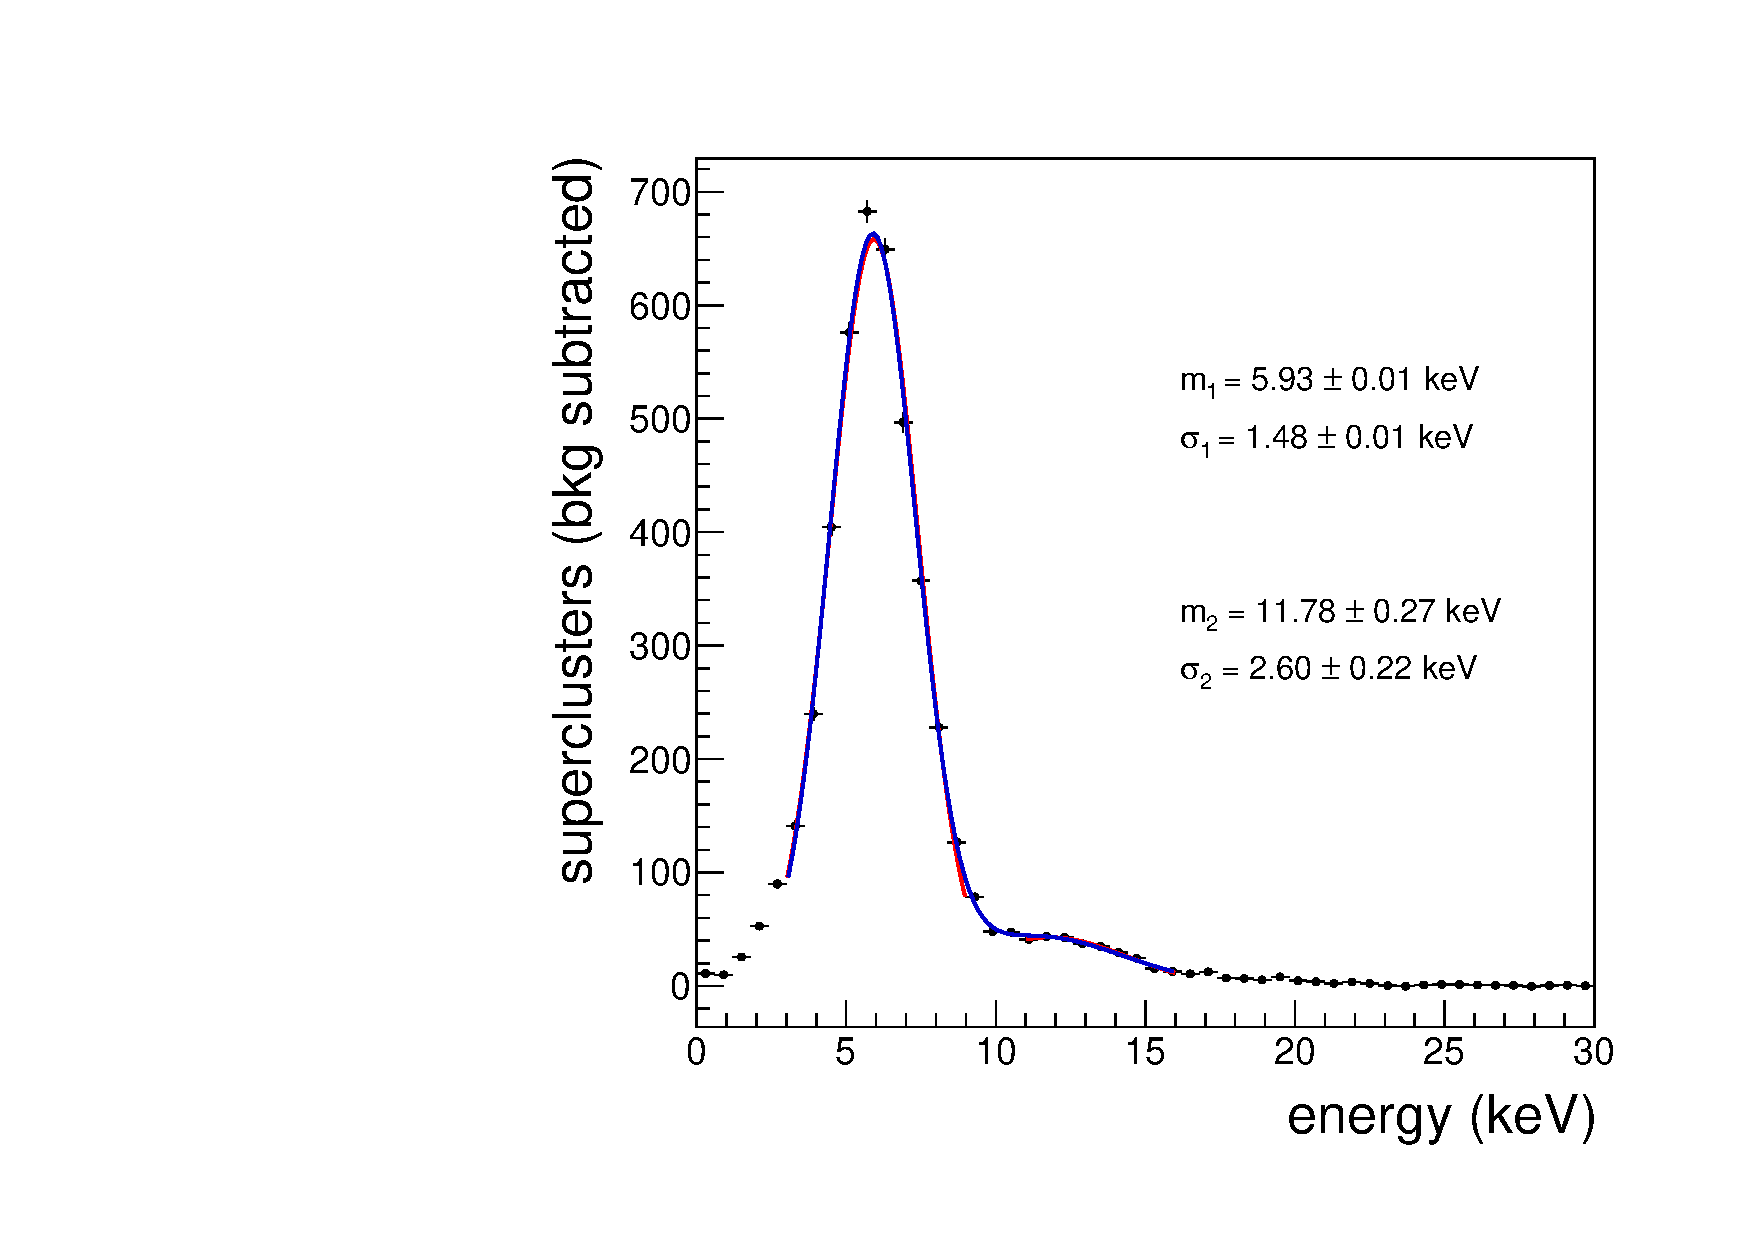
\includegraphics[width=0.49\linewidth]{figures/fe_energy_fit}
%%     \caption{Distribution of the supercluster energy, calibrated with
%%       the procedure described in the text, in events with the \fe
%%       source. Clearly visible is the large peak of a single spot, and,
%%       at around twice the energy, a broader peak for the case of two
%%       neighbor spots merged in a single supercluster.
%%       \label{fig:fepeak}}
%%   \end{center}
%% \end{figure}
%

The skeletonization procedure provides a general method to estimate
the track length ($l_p$), which is accurate both in the case of straight
and curving track.  In the case of straight tracks, the length extracted
in this way coincides with the major axis estimated with a principal
component analysis (PCA), described in the following section. For
exactly round spots, the skeleton would collapse in the center of the
cluster and the resulting length would be 1 pixel, but this completely
symmetric case never happens in the considered samples.
